\section{Scope: Global, Function, dan Block}

\textbf{Scope} menentukan di mana variabel dapat diakses dalam program. JavaScript memiliki tiga level scope: \textbf{global} (variabel tersedia di mana saja), \textbf{function} (variabel hanya tersedia di dalam fungsi tempat dideklarasikan), dan \textbf{block} (variabel hanya tersedia di dalam blok \code{\{ \}} tempat dideklarasikan). \code{var} mengikuti function scope, sedangkan \code{let} dan \code{const} mengikuti block scope \cite{jsInfo}.

\begin{figure}[htbp]
\centering
\resizebox{0.8\textwidth}{!}{%
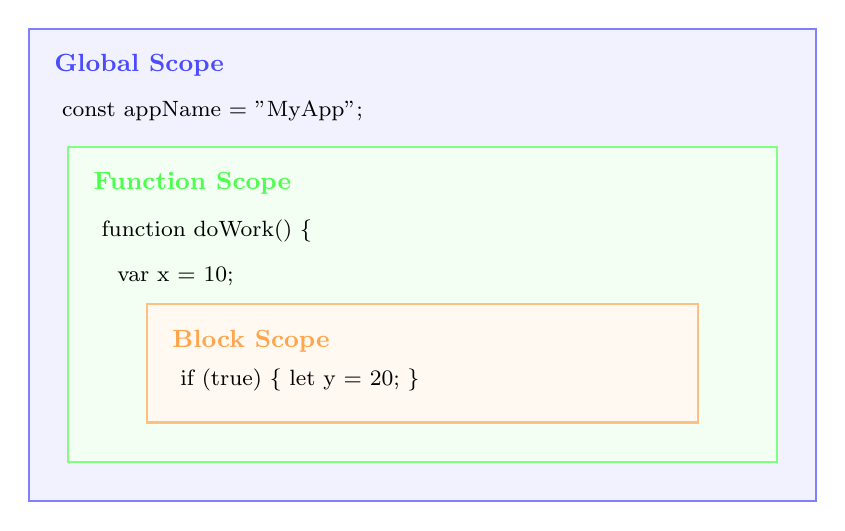
\begin{tikzpicture}[every node/.style={font=\footnotesize}]
  % Global scope
  \draw[thick, blue!50, fill=blue!5] (0,0) rectangle (10,6);
  \node[anchor=north west, font=\small\bfseries, blue!70] at (0.2,5.8) {Global Scope};
  \node[anchor=north west] at (0.3,5.2) {\code{const appName = "MyApp";}};
  % Function scope
  \draw[thick, green!50, fill=green!5] (0.5,0.5) rectangle (9.5,4.5);
  \node[anchor=north west, font=\small\bfseries, green!70] at (0.7,4.3) {Function Scope};
  \node[anchor=north west] at (0.8,3.7) {\code{function doWork() \{}};
  \node[anchor=north west] at (1.0,3.1) {\code{var x = 10;}};
  % Block scope
  \draw[thick, orange!50, fill=orange!5] (1.5,1) rectangle (8.5,2.5);
  \node[anchor=north west, font=\small\bfseries, orange!70] at (1.7,2.3) {Block Scope};
  \node[anchor=north west] at (1.8,1.8) {\code{if (true) \{ let y = 20; \}}};
\end{tikzpicture}%
}
\caption{Tiga level scope di JavaScript: global, function, dan block}
\end{figure}

\textbf{Closure} terjadi ketika fungsi ``mengingat'' variabel dari scope luar tempat ia diciptakan, bahkan setelah fungsi luar selesai dieksekusi. Closure adalah konsep kunci untuk memahami callback, factory function, dan banyak pola JavaScript. Variabel dalam closure tetap hidup selama fungsi yang mereferensinya masih ada \cite{mdnJsGuide}.

\begin{konsep}
\textbf{Hindari Variabel Global.} Variabel global dapat diakses dan diubah dari mana saja---ini menciptakan ``polusi namespace'' dan bug yang sulit dilacak. Minimalkan variabel global: bungkus kode dalam fungsi atau modul. Gunakan \code{let}/\code{const} yang block-scoped, bukan \code{var} yang function-scoped. Dalam proyek modern, ES6 modules (\code{import}/\code{export}) secara otomatis membatasi scope ke file \cite{jsInfo}.
\end{konsep}

